\section{Summary of SCOC Phase 3 recommendations}\label{sec:summary}
The following list summarizes the Phase 3 recommendations for the LSST survey strategy which together with the recommendations in \citetalias{PSTN-053} and \citetalias{PSTN-055} define the LSST survey strategy starting plan.   The recommendations included in this report are listed below.

\begin{itemize}
\item The SCOC recommends swapping $u$- and $y$-band according to the moon phase. Having the $z$ filter always available  produces benefits for SN cosmology while preserving coverage on short timescales. This recommendation is implemented starting in \baseline{3.2} (\autoref{sec:filterswap}).




\item All three mirrors in the system will now be coated in silver, which increases throughput in all bands bluer than $u$ but decreases $u$ throughput (by $\lesssim30\%$). Hence, the SCOC recommends an increase of the exposure time in $u$-band to 38 seconds per visit and an increase of the number of $u$-band visits of 10\% compared to \baseline{3.0}. To compensate for the additional time dedicated to $u$ band the SCOC recommends decreasing the exposure time in the other bands. Simulations show that this corresponds to a decrease of 0.8 second exposure time per visit in all other bands (\autoref{sec:filterbalance}).

\item {The SCOC confirms the recommendation for rolling in two sky areas at 0.9 strength on the WFD low-dust footprint (\citetalias{PSTN-055} Section 2.5). We are adopting the rolling uniform strategy designed by the Uniformity Task Force in \baseline{3.6} simulations, which implements three cycles of rolling, but we will continue to investigate implementations of rolling until our Y1 recommendation since rolling will not begin before the start of Y2 with any of the implementations under consideration.  The SCOC recommends that the time domain community, particularly those interested in phenomena that have evolutionary time scales of hours-to-days, urgently quantifies the impact of the proposed uniform rolling compared to rolling in four cycles. Further, the SCOC restates the recommendation that Data Management scopes a plan for producing uniform data releases in DR5 and DR8 in addition to the standard data releases and that the cost of the development and storage of these additional data releases is scoped and shared with the scientific community (\autoref{sec:rolling}).} 

\item The SCOC concludes that rolling on the Galactic footprint would have a net negative effect on the survey as a whole, and recommends no rolling in the Plane or Bulge (\autoref{sec:subG:footprint}).


\item The SCOC recommends redistributing the visits concentrated in the ``blob'' centered around a Galactic longitude of $l=+45$ (see \autoref{fig:gpfootprint}, top) to cover a low-visit ``barrier'' at $l=+335$ in the Plane and at the border of the Plane and Bulge. This change would give continuous longitude coverage along the Plane from a longitude of $l=+30$  through $l=+280$ and boost metrics for time-domain science in the Bulge/Plane (\autoref{sec:subG:footprint}).

\item The SCOC recommends a visit plan consistent with the \texttt{roman\_v3.3} simulation, capping the number of visits redistributed to the Roman Bulge field at the value ($\sim 1600$) used in this simulation. However, the timing of the implementation of this augmented observing campaign should remain flexible to respond to the final Roman launch date and survey scheduling (\autoref{sec:subG:footprint}).

\item The SCOC finds that the adoption of a revised filter balance in the Bulge and Plane with less $y$ and more $z$, $g$, and $u$ compared to the present baseline is potentially beneficial for a broad range of science, but that existing metrics are not adequately sensitive to the explored filter balance changes for some expected science cases. The SCOC concludes that a survey using the currently implemented filter balance in the Bulge and Plane in \baseline{3.4} will produce excellent science and the LSST can start with this implementation (\autoref{sec:subG:filterbalance}).

\item The SCOC recommends a bluer filter mix in the SMC, LMC, and SCP regions, bounded by the requirement that the increased number of dark-time visits in a relatively narrow range of right ascension does not affect other parts of the survey (\autoref{sec:subG:specialregions}).

\item The SCOC recommends the implementation of an LSST ToO program as detailed in \emph{Rubin ToO 2024: 
Envisioning the Vera C. Rubin Observatory LSST Target of Opportunity program
}\footnote{\url{https://docs.google.com/document/d/1WE4NGl3dFOVGo7lzpyG1fe_JiX9m-kLl5JYQkhu9iso/edit?usp=sharing}} by the scientific community at large (\autoref{sec:ToO}).

\item The SCOC recommends that a meeting to follow Rubin ToO 2024 is organized closer to the start of the LKV O5 run (expected 2027) to refine the GW follow-up survey strategy with improved knowledge of the expected performance of the GW detector networks and systems in O5 and of the performance of the full Rubin system. In addition, solar system and neutrino ToOs should start as soon as suitable templates are available (\autoref{sec:ToO}).

\item The SCOC recommends that Rubin only consider potential ToOs that emanate from vetted discovery and distribution systems that produce and dispatch fully machine-readable alerts (\autoref{sec:ToO}).

\item The SCOC recommends real-time human review of potential ToO triggers and the establishment of a Rubin ToO Advisory Committee as described above (\autoref{sec:ToO}).

\item The SCOC recommends that, if the technical feasibility is confirmed in commissioning, the survey is conducted with single exposures. With our recommendation of modifying the exposure time for $u$ band to 38 seconds, and compensating for this extra $u$ band survey time by short decrease in exposure across all other bands, the single visits would be 1x29.2 seconds (\autoref{sec:snaps}).

\item The SCOC recommends that DDF observations should be sequences of multiple WFD-like visits (as opposed to increased exposure times) to allow rapid alert generation (\autoref{sec:DDF}).

\item The SCOC recommends that the baseline translational dithering scale of DDF observations should be reduced from 0.7 degrees to 0.2 degrees (with exploration of even smaller translational dithers compatible with instrumental signature removal and calibration needs). (\autoref{sec:DDF}).

\item The SCOC recommends that the baseline survey strategy should accommodate varying the nightly depth, filters, or cadence of different DDFs throughout the course of LSST, while maintaining the Phase 2 recommendations for the 10-year depth of each field (including the enhanced COSMOS observations to reach 10-year depth in the first 3 years) (\autoref{sec:DDF}).

\item The SCOC urges the Data Management and Alert Production teams to assess the feasibility of, and resources needed for, enabling nightly co-adds of sequential DDF visits and recommends that a path is developed to enable the creation of these co-adds, subtraction with deep templates, and faint alert generation (with higher latency as needed, \eg , after sunrise) (\autoref{sec:DDF}). 

\item The SCOC recommends that the airmass limit for the Near-Sun Twilight microsurvey is increased to $X=3.0$ (\autoref{sec:additional}).

\item The SCOC recommends a slight modification of the \baseline{3.0} footprint to improve overlap with the Euclid footprint (\autoref{sec:additional}). 

\end{itemize}

These recommendations will be implemented in the \baseline{4.0} simulations. A set of simulations tagged \texttt{v3.6} is made available for the community to assess the impact of different aspects of the recommendation. Note that all of these simulations include the updated, more realistic downtime and effects of slew jerk. 

 \autoref{fig:summary} shows the performance of the survey strategy on a set of core LSST science and system metrics. Note: Significant improvements were obtained on most metrics through v3.0. Those are to be attributed to changes of the survey strategy through community input and SCOC recommendations. The visible improvement on nearly all metrics between \baseline{3.2} and \baseline{3.3} is attributed to the updated filter transmission curves. The survey strategy is largely unchanged between \baseline{3.3} and \baseline{3.4}; the small changes in performance are to be attributed to  \texttt{rubin\_scheduler} code updates.\footnote{See \url{https://survey-strategy.lsst.io/baseline/changes.html}}. \baseline{3.6} reflects the recommendations described in this document. The overall apparent drop in performance between \baseline{3.4} and \baseline{3.6} is primarily due to the inclusion of slew time jerk effects and more realistic estimates of downtime in Y1 (\autoref{sec:opsimchanges}). While \baseline{3.6} has three rolling cycles, we also make available a variation of \baseline{3.6} with four cycles of rolling to enable the investigations of different rolling implementations. While our recommendation is to implement the ToO program as described in \autoref{sec:ToO}, we provide an \opsim\ consistent with \baseline{3.6}, but without the ToO program to allow the community, to see the small effects that the introduction of ToOs has on the LSST. Finally we provide an implementation of \baseline{3.6} with single exposure visits (instead of 2x15 second snaps, \autoref{sec:snaps}) which, pending commissioning outcomes, is the expected observing mode. In this \opsim, the survey time gained by dropping snaps (decreased readtime per visit) is allocated evenly across all all-sky observing modes: this includes the WFD, NES, SCP and Galactic Plane.


\begin{figure}
    \centering
    \begin{overpic}[width=0.8\textwidth]{figures/scoc_heatmap.png}
        	\put(50,50){\color{lsstblue}\huge DRAFT}
    \end{overpic}
    %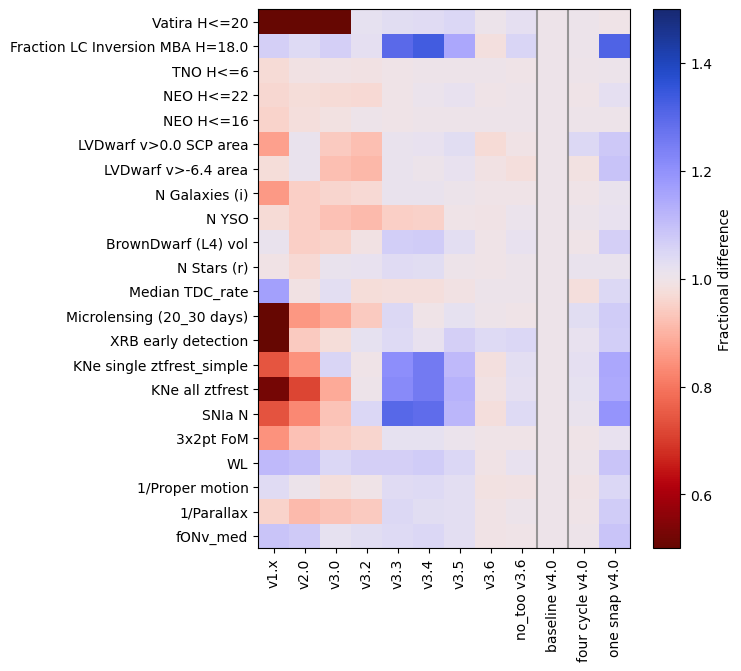
\includegraphics[width=0.9\linewidth]{figures/scoc_heatmap.png}
    \caption{LSST performance on key metrics for different \opsim s including the Phase 3 recommendation (this document). From left to right, then sequence shows progressively newer \opsim s, starting with the baseline in effect through 2018 (\texttt{v1.x}) up to the baseline proposed with this recommendation (\baseline{3.6}) and some variations on the latter. Starting with \baseline{3.6} we include more realistic down time expectations in Y1 and the effects of slew jerk on scheduling and observing. This causes an overall decreass in the number of visits (see also \autoref{fig:nvisits}). \baseline{3.6} is also the first \opsim\  shown here which includes the ToO program. Rolling is implemented in 3 cycles in \baseline{3.6}. This achieves desired uniformity in DR5 and DR8 (see \autoref{sec:rolling}). \texttt{four cycles} implements rolling in four cycles. The SCOC will not commit to a recommendation on the specific rolling implementation until the release of its Y1 recommendation. The community is encouraged to explore the impact of adopting either rolling strategy on their science. A version of \baseline{3.6} without ToO (\texttt{no ToO}) is included to allow the community to see the impact of the ToO program but the SCOC is committed to recommending the implementation of a ToO program as simulated in \baseline{3.6}. Finally, we include an implementation of \baseline{3.6} where visits are conducted in a single exposure instead of two snaps (\texttt{single snap}). The SCOC recommends the implementation of LSST in single visits (as shown in this simulation); this recommendation is, however, pending commissioning outcomes.}
    \label{fig:summary}
\end{figure}

\begin{figure}
    \centering
    \begin{overpic}[width=0.8\textwidth]{figures/total_nvisits.png}
        	\put(50,30){\color{lsstblue}\huge DRAFT}
    \end{overpic}
    %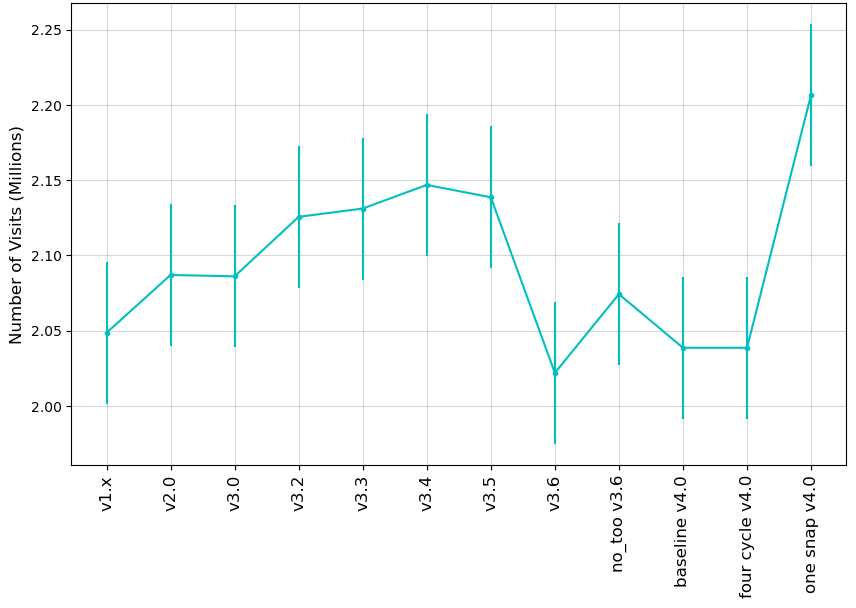
\includegraphics[width=0.5\linewidth]{figures/total_nvisits.png}
    \caption{Number of LSST visits for the same set of \opsim s used in \autoref{fig:summary}. The number of observations decreses between \texttt{v3.4} and \baseline{3.6} because of the inclusion of more realistic down times in Y1, of the effects of jerk on slew and scheduling, and, in part, because of the inclusion of the ToO program in LSST. This drop in number of visit determines a general loss of performance on all metrics, as seen in \autoref{fig:summary}. The increase in efficiency associated with moving to single exposure visits (the \opsim\ labeled as \texttt{single snaps}) largely recovers the visits lost between \texttt{3.4} and \baseline{3.6}. Nonetheless, after Y1, when the system performance is better understood, n the future, the SCOC will consider how the additional time may be allocated (\autoref{sec:snaps}). }
    \label{fig:nvisits}
\end{figure}

\FloatBarrier
